\documentclass[landscape]{article}

%%%%%%%%%%%%%%%%%%%%%%%%%%%%%%%%%
% PACKAGES
%%%%%%%%%%%%%%%%%%%%%%%%%%%%%%%%%

\usepackage{acronym,amsthm,babel,boxedminipage,longtable,fancyhdr,framed, mathtools,amsmath, amssymb,
  colortbl,epsfig,lscape,multirow,setspace,tabularx,titlesec,subcaption,graphicx,%tweaklist,
  moreverb,xcolor,xspace}

\usepackage[
bookmarks,bookmarksopen,bookmarksnumbered,bookmarksopenlevel=2,
pdftitle=Streaming\ NMT\ from\ English\ into\ EU\ languages,%
citebordercolor=blue,
filebordercolor=teal,
linkbordercolor=lightgray,
menubordercolor=violet,
urlbordercolor=lightgray,
runbordercolor=darkgray]{hyperref}

\usepackage{alltt,amsmath,boxedminipage,calc,datetime,dcolumn,ifthen,
                   moreverb,multido,pifont,rotating,tabularx}
                   
\usepackage[utf8]{inputenc}
\usepackage{mllp}
\graphicspath{{../figures/}{figures/}}
\usepackage{tikz}
\usepackage{graphicx}
%\usepackage{subfig}
\usepackage{pgfplots}
\usepackage[eulergreek]{sansmath}
\usetikzlibrary{arrows,shapes,snakes,automata,backgrounds,petri,calc,fit,positioning}

\usepackage{scalerel,stackengine}
\usepackage{float}

\DeclarePairedDelimiter\ceil{\lceil}{\rceil}
\DeclarePairedDelimiter\floor{\lfloor}{\rfloor}

\newcommand\bunderline[1][\budefaultcolor]{\def\bucolor{#1}\bunderlineaux}
\newcommand\bunderlineaux[2][\buthickness]{%
  \ThisStyle{%
  \ifmmode%
    \setbox0=\hbox{\m@th$\SavedStyle#2$}
    \stackunder[2pt]{\copy0}{\textcolor{\bucolor}{\rule{\wd0}{#1}}}%
  \else%
    \xdef\butmpthickness{#1}%
    \prebunderlinewords#2 \endarg%
  \fi%
}}
\def\prebunderlinewords#1 #2\endarg{%
  \ifx\endarg#2\endarg\def\wdaugment{0pt}\else\def\wdaugment{.8ex}\fi%
  \bunderlinewords#1 #2\endarg%
}
\def\bunderlinewords#1 #2\endarg{%
    \setbox0=\hbox{#1\strut}%
    \stackengine{0pt}{\copy0}{\textcolor{\bucolor}{%
      \smash{\rule{\dimexpr\wd0+\wdaugment\relax}{\butmpthickness}}}}{U}{c}{F}{T}{S}% 
    \ifx\endarg#2\endarg\def\next{}\else\ \def\next{\bunderlinewords#2\endarg}\fi\next%
}
\newcommand\buonslide[1][black]{\def\butmpcolor{#1}\buonslideauxA}
\newcommand\buonslideauxA[1][\buthickness]{\def\butmpthickness{#1}\buonslideauxB}
\def\buonslideauxB<#1>#2{\onslide<#1>{%
  \rlap{\bunderline[\butmpcolor][\butmpthickness]{\phantom{#2}}}}#2}



%%%%%%%%%%%%%%%%%%%%%%%%%%%%%%%%%
% HEADERS & FOOTERS
%%%%%%%%%%%%%%%%%%%%%%%%%%%%%%%%%

\pagestyle{plain}

\renewcommand{\today}{21 September, 2022}

\renewcommand{\author}{Guillem Calabuig Domenech}
\renewcommand{\authorshort}{Guillem Calabuig}
\renewcommand{\title}{Streaming neural machine translation systems from English into European languages}
\renewcommand{\titleshort}{Streaming NMT from English into European languages}

%%%%%%%%%%%%%%%%%%%%%%%%%%%%%%%%%
% COLORS
%%%%%%%%%%%%%%%%%%%%%%%%%%%%%%%%%

\definecolor{mygrey}{gray}{.75}
\definecolor{gray}{rgb}{0.9,0.9,0.9}
\definecolor{drakgray}{rgb}{0.34,0.35,0.32}
\definecolor{darkred}{rgb}{0.71,0.13,0.14}
\definecolor{darkgreen}{rgb}{0.2,0.5,0.3}
\definecolor{greygreen}{rgb}{0.25,0.5,0.25}
\definecolor{greyblue}{rgb}{0.34,0.34,0.42}
\definecolor{darkblue}{rgb}{0.1,0.2,0.6}
\definecolor{darkmagenta}{rgb}{.55,0,.55}

%%%%%%%%%%%%%%%%%%%%%%%%%%%%%%%%%
% SUBSUBSUBSECTION
%%%%%%%%%%%%%%%%%%%%%%%%%%%%%%%%%

\setcounter{secnumdepth}{1} % section numbering is applied up to this level
\setcounter{tocdepth}{2} % sections up to given depth are included in toc


%%%%%%%%%%%%%%%%%%%%%%%%%%%%%%%%%
% DOCUMENT
%%%%%%%%%%%%%%%%%%%%%%%%%%%%%%%%%

\begin{document}

%%%%%%%%%%%%%%%%%%%%%%%%%%%%%%%%%
% TITLE PAGE
%%%%%%%%%%%%%%%%%%%%%%%%%%%%%%%%%

\thispagestyle{empty}

\begin{center}

\centerline{
\includegraphics[height=0.15\textheight]{figures/UPV-logo}}

\rule{0mm}{20mm}
\Large{\setstretch{1.5}\Large\textbf{\color{darkred}\title}}

\rule{0mm}{30mm}
{\normalsize \color{greyblue}\author}

\newcolumntype{Y}{>{\centering\arraybackslash}X}
\rule{0mm}{0mm}
\begin{table}[ht!]
    \begin{tabularx}{\textwidth}{YY}
        \small \color{greyblue} Jorge Civera Saiz & \small \color{greyblue} Javier Iranzo Sánchez\\
    \end{tabularx}
\end{table}

\end{center}

\centerline{
\includegraphics[height=0.12\textheight]{figures/MLLP_Brand} \qquad \qquad 
\includegraphics[height=0.15\textheight]{figures/vrain.png}}

\normalsize\small
\vspace{10mm}

\centerline{\today}
\vfill

\clearpage

%%%%%%%%%%%%%%%%%%%%%%%%%%%%%%%%%
% TABLE OF CONTENTS
%%%%%%%%%%%%%%%%%%%%%%%%%%%%%%%%%
 
\hypertarget{INDEX}{}

\tableofcontents

%%%%%%%%%%%%%%%%%%%%%%%%%%%%%%%%%
% INTRODUCTION: MOTIVATION & FRAMEWORK
%%%%%%%%%%%%%%%%%%%%%%%%%%%%%%%%%

%\cp 
%\section{Introduction}
%\vspace*{10mm}
%\subsection*{Motivation}
%\vspace*{5mm}
%\begin{itemize}\itemsep=5mm
%	\item Increase accessibility of multimedia content to non-speakers of the original language
%	\item Remove language barriers in virtual meetings and video-conferences in real time
%\end{itemize}
%
%\subsection*{Framework}
%\vspace*{5mm}
%\begin{itemize}\itemsep=5mm
%	\item Research internship at the VRAIN MLLP research group
%	\item Technology-transfer contract between MLLP and CERN
%	\begin{itemize}
%		\item En$\to$Fr machine translation (MT) systems for offline and real-time scenarios
%	\end{itemize}
%\end{itemize}

%%%%%%%%%%%%%%%%%%%%%%%%%%%%%%%%%
% INTRODUCTION: GOALS
%%%%%%%%%%%%%%%%%%%%%%%%%%%%%%%%%

\cp
\section{Introduction}
\vspace*{10mm}
\subsection*{Goals}
\vspace*{5mm}
 \begin{itemize}\itemsep=5mm
     \item To understand the theoretical developments and technological advances that have led neural machine translation (NMT) to be the current state of the art.
    \item To learn and showcase the different components and processes involved in the development of NMT systems, as well as the importance of data and how it is compiled for these systems.
    \item To improve the offline NMT models for the English to French translation task that already exist in the MLLP research group.
    \item To explore, compare and apply different methods to adapt NMT systems to a specific domain in order to significantly improve the translation quality in in-domain evaluation tasks.
    \item To understand the challenges that exist in building streaming and real time NMT models, how they are evaluated, and construct a system for such task based on offline system results.
    \item To develop MT systems ready to be deployed and used in real scenarios for the English to French translation task.
\end{itemize}

%%%%%%%%%%%%%%%%%%%%%%%%%%%%%%%%%
% PRELIMINARIES: MT
%%%%%%%%%%%%%%%%%%%%%%%%%%%%%%%%%

\cp
\section*{Introduction}
\vspace*{10mm}
\subsection*{Machine Translation}
\vspace{5mm}
\begin{itemize}
	\item In MT, we search for the best translation $\mathbf{\hat{y}}$ of $\mathbf{x}$ given by
\end{itemize}
\vspace{5mm}
\begin{equation}\nonumber
	\mathbf{\hat{y}}=\argmax_{\mathbf{y} \in \mathcal{Y^*}} p(\mathbf{y}|\mathbf{x})
\end{equation}
\vspace*{5mm}
\begin{itemize}\itemsep=5mm
	\item $\mathbf{x}$ is the \textit{source} sentence and $\mathbf{y}$ is the \textit{target} sentence
	\item The neural models we will use approximate $p(\mathbf{y}|\mathbf{x})$ directly
%	\item The \textit{beam search} algorithm is used to instantiate the argmax
\end{itemize}

%%%%%%%%%%%%%%%%%%%%%%%%%%%%%%%%%
% PRELIMINARIES: MLP, TRANSFORMER
%%%%%%%%%%%%%%%%%%%%%%%%%%%%%%%%%

\cp
\section*{Introduction}
\vspace*{10mm}
\subsection*{Transformer}
\vspace*{-12mm}
\minipage{0.35\textwidth}
\begin{itemize}\itemsep=7mm
	\item Deep learning architecture based on the \textit{attention} mechanism
	\item State-of-the-art in many NLP tasks
    \item Softmax giving output probabilities from which output phrase is computed 
\end{itemize}
\endminipage\hfill
\minipage{0.6\textwidth}
\vspace{4mm}
\centering
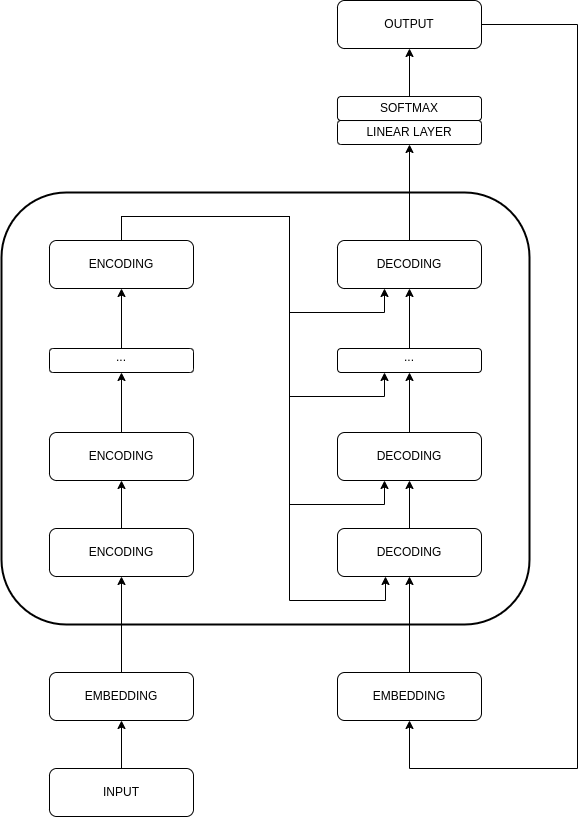
\includegraphics[scale=0.5]{../memoria/resources/transformer.png}
\endminipage\hfill

%%%%%%%%%%%%%%%%%%%%%%%%%%%%%%%%%
% INTRODUCTION: EVALUATION 
%%%%%%%%%%%%%%%%%%%%%%%%%%%%%%%%%

\cp
\section*{Introduction}
\vspace*{10mm}
\subsection*{Evaluation}
\vspace*{5mm}
\begin{itemize} \itemsep=5mm
	\item Manual evaluation is very costly
	\item Automatic evaluation
	\begin{itemize}
		\item \empha{BLEU: Bilingual Evaluation Understudy} $\to$ Higher is better
	\end{itemize}
\end{itemize}
\vspace*{-5mm}
%\subsection*{Tools}
%\vspace*{5mm}
%\begin{itemize}
%\item Model training and inference: fairseq
%\item Data processing: Moses, subword-nmt, SentencePiece, etc.
%\end{itemize}

\subsection*{Framework}
\vspace*{5mm}
\begin{itemize}\itemsep=5mm
	\item Research internship at the VRAIN MLLP research group
	\item Technology-transfer contract between MLLP and CERN
	\begin{itemize}
		\item En$\to$Fr MT systems for offline and real-time scenarios
	\end{itemize}
\end{itemize}

%%%%%%%%%%%%%%%%%%%%%%%%%%%%%%%%%
% DATA: GENERAL DOMAIN
%%%%%%%%%%%%%%%%%%%%%%%%%%%%%%%%%

\cp
\section{Data}
\vspace*{10mm}
\subsection*{Training Dataset}
\vspace*{5mm}
\begin{table}[!ht]
\centering
\begin{tabular}{c|l||r|r|r} 
Source&Corpus						&		Bilingual pairs		&		\multicolumn{2}{c}{Words}		\\	
		&					&									&		English			&			French			\\	\hline	
&WikiMatrix				&		2.7 M					&		57.8 M			&			63.1 M			\\ 
&WikiMedia				&		1.0 M					&		24.1 M			&			25.8 M			\\ 
&Giga	Fr-En					&		22.5 M					&		575.8 M		&			672.2 M		\\ 
&ParaCrawl					&		216.6 M				&		3.7 G				&			4.1 G				\\ 
Internet&CCAligned					&		15.6 M					&		156.7 M		&			171.1 M		\\ 
&CommonCrawl			&		0.1 M					&		4.1 M			&			4.7 M		 	\\
&EUBookshop 			&		10.8 M					&		224.6 M		&			244.5 M		\\  
&UNPC						&		30.3 M					&		658.4 M		&			816.4 M		\\ 
&News Commentary 	&		3.2 M					&		70.7 M			&			76.6 M			\\ \hline 
&DGT-TM					&		4.9 M					&		86.3 M			&			95.4 M			\\ 
Parliamentary&Europarl					&		1.2 M					&		28.6 M			&			29.9 M			\\ 
Meetings&Europarl-ST 				&		96.5 K 					&		2.3 M			&			2.6 M 			\\ \hline
&Total							&		\textbf{309.0 M}				&		5.6 G				&			6.3 G				\\ 
\end{tabular}
\end{table}

%%%%%%%%%%%%%%%%%%%%%%%%%%%%%%%%%
% DATA: IN-DOMAIN
%%%%%%%%%%%%%%%%%%%%%%%%%%%%%%%%%

%\cp
%\section*{Training Data}
%\vspace*{10mm}
%\subsection*{Domain of CERN}
%\vspace*{5mm}
%\subsubsection*{Monolingual CDS Corpus}
%\begin{table}[!ht]
%\centering
%\begin{tabular}{l|rrrr}
% 						&		Objects		 	&		Sentences					& Words		\\ \hline
%Titles 				&		519 K			&		519.0 K 					&	4.6 M		\\
%Abstracts			&		130 K			&		652.0 K						&	15.6 M		\\
%Documents		&		296 K 			&		48.9 M 						&	1.1 G			\\ \hline
%Total					&		945 K			& 		\textbf{50.0 M}			&	1.1 G 		\\
%
%\end{tabular}
%\end{table}



%%%%%%%%%%%%%%%%%%%%%%%%%%%%%%%%%
% DATA: PROCESSING STEPS
%%%%%%%%%%%%%%%%%%%%%%%%%%%%%%%%%

\cp
\section*{Data}
\subsection*{Data Processing}
\begin{itemize}\itemsep=5mm
	\item Filtering $\to$ Remove low quality sentences / Reduce noise in data 
		\begin{itemize}
		\item Language identification
		\item Source-to-Target length ratio
		\end{itemize}
	\item Tokenization $\to$ Divide text into \textit{tokens}
	\item Truecasing $\to$ Maintain the most frequent version of each token
	\item Subword Segmentation $\to$ Mimic an open vocabulary using token segments
		\begin{itemize}
			\item Byte-Pair Encoding
			\item SentencePiece
		\end{itemize}

\end{itemize}
\begin{table}[ht]
\centering
\resizebox{23cm}{3.2cm}{
\begin{tabular}{|c|l|c}
\hline
    Original & Mrs Plooij-van Gorsel, I can tell you that this matter is on  \\
    
    sentence & is on the agenda for the Quaestors' meeting on Wednesday.\\
\hline
    Truecased and & Mrs Plooij @-@ van Gorsel , I can tell you that this matter is on\\
    tokenized & the agenda for the Quaestors ' meeting on Wednesday .\\
\hline
    Truecased, tokenized & Mrs P@@ loo@@ i@@ j @-@ van Gor@@ sel , I can tell you  \\
    and BPE encoded & that this matter is on the agenda for the Qu@@ a@@ \\
    sentence & est@@ ors ' meeting on Wednesday .\\
    \hline
    Truecased and & Mrs\_ P loo ij - van\_ Gor sel ,\_ I\_ can\_ tell\_ you\_ that\_ this\_ \\
    SPM encoded & matter\_ is\_ on\_ the\_ agenda\_ for\_ the\_ Qu a est ors '\_  \\
    sentence & meeting\_ on\_ Wednesday .\_ \\
\hline
\end{tabular}}
\end{table}


\cp
\section{CERN News Corpus}
\subsection*{Corpus Compilation}
\begin{itemize}
    \item{Crawling $\to$ Source contents from CERN website}
    \item{Alignment $\to$ Transform raw text to parallel documents}
        \begin{itemize}
            \item{Split lines (MOSES)}
            \item{Hunalign}
        \end{itemize}
    \item{Manual Revision $\to$ Assure semantic meaning matches in both languages}
\end{itemize}



\subsection*{Bilingual CERN News Corpus}
\begin{table}[ht]
\centering
\begin{tabular}{l|c|c|c}
& Sentence pairs & English words & French words \\
\hline
    CN21 & 2200 & 53.4K & 60.8K \\
    CN22 & 1799 & 44K & 49.9K \\
\hline
    CNTraining & 55943 & 1230K & 1395K \\
    CNTraining90 & 50340 & 1090K & 1228K \\
    CNTraining70 & 39150 & 891K & 1000K \\
    CNTraining50 & 27971 & 615K & 688K \\
\hline

\end{tabular}
\label{table:cnstats}
\end{table}

%%%%%%%%%%%%%%%%%%%%%%%%%%%%%%%%%
% DOMAIN ADAPTATION: BT & FT
%%%%%%%%%%%%%%%%%%%%%%%%%%%%%%%%%
\cp
\section{Offline systems}
\vspace*{10mm}
\subsection*{Fairseq}
\begin{itemize}
    \item Facebook AI research implementation of Transformer model (binarize, training, averaging, inference) 
\end{itemize}

\vspace*{10mm}
\subsection*{Offline scenario}
\begin{itemize}
    \item Consider the full input sentence when computing target sentence
    \item No time cost is considered 
\end{itemize}

\cp
\section*{Offline systems}
\subsection*{Versions}
\vspace*{10mm}
\centering
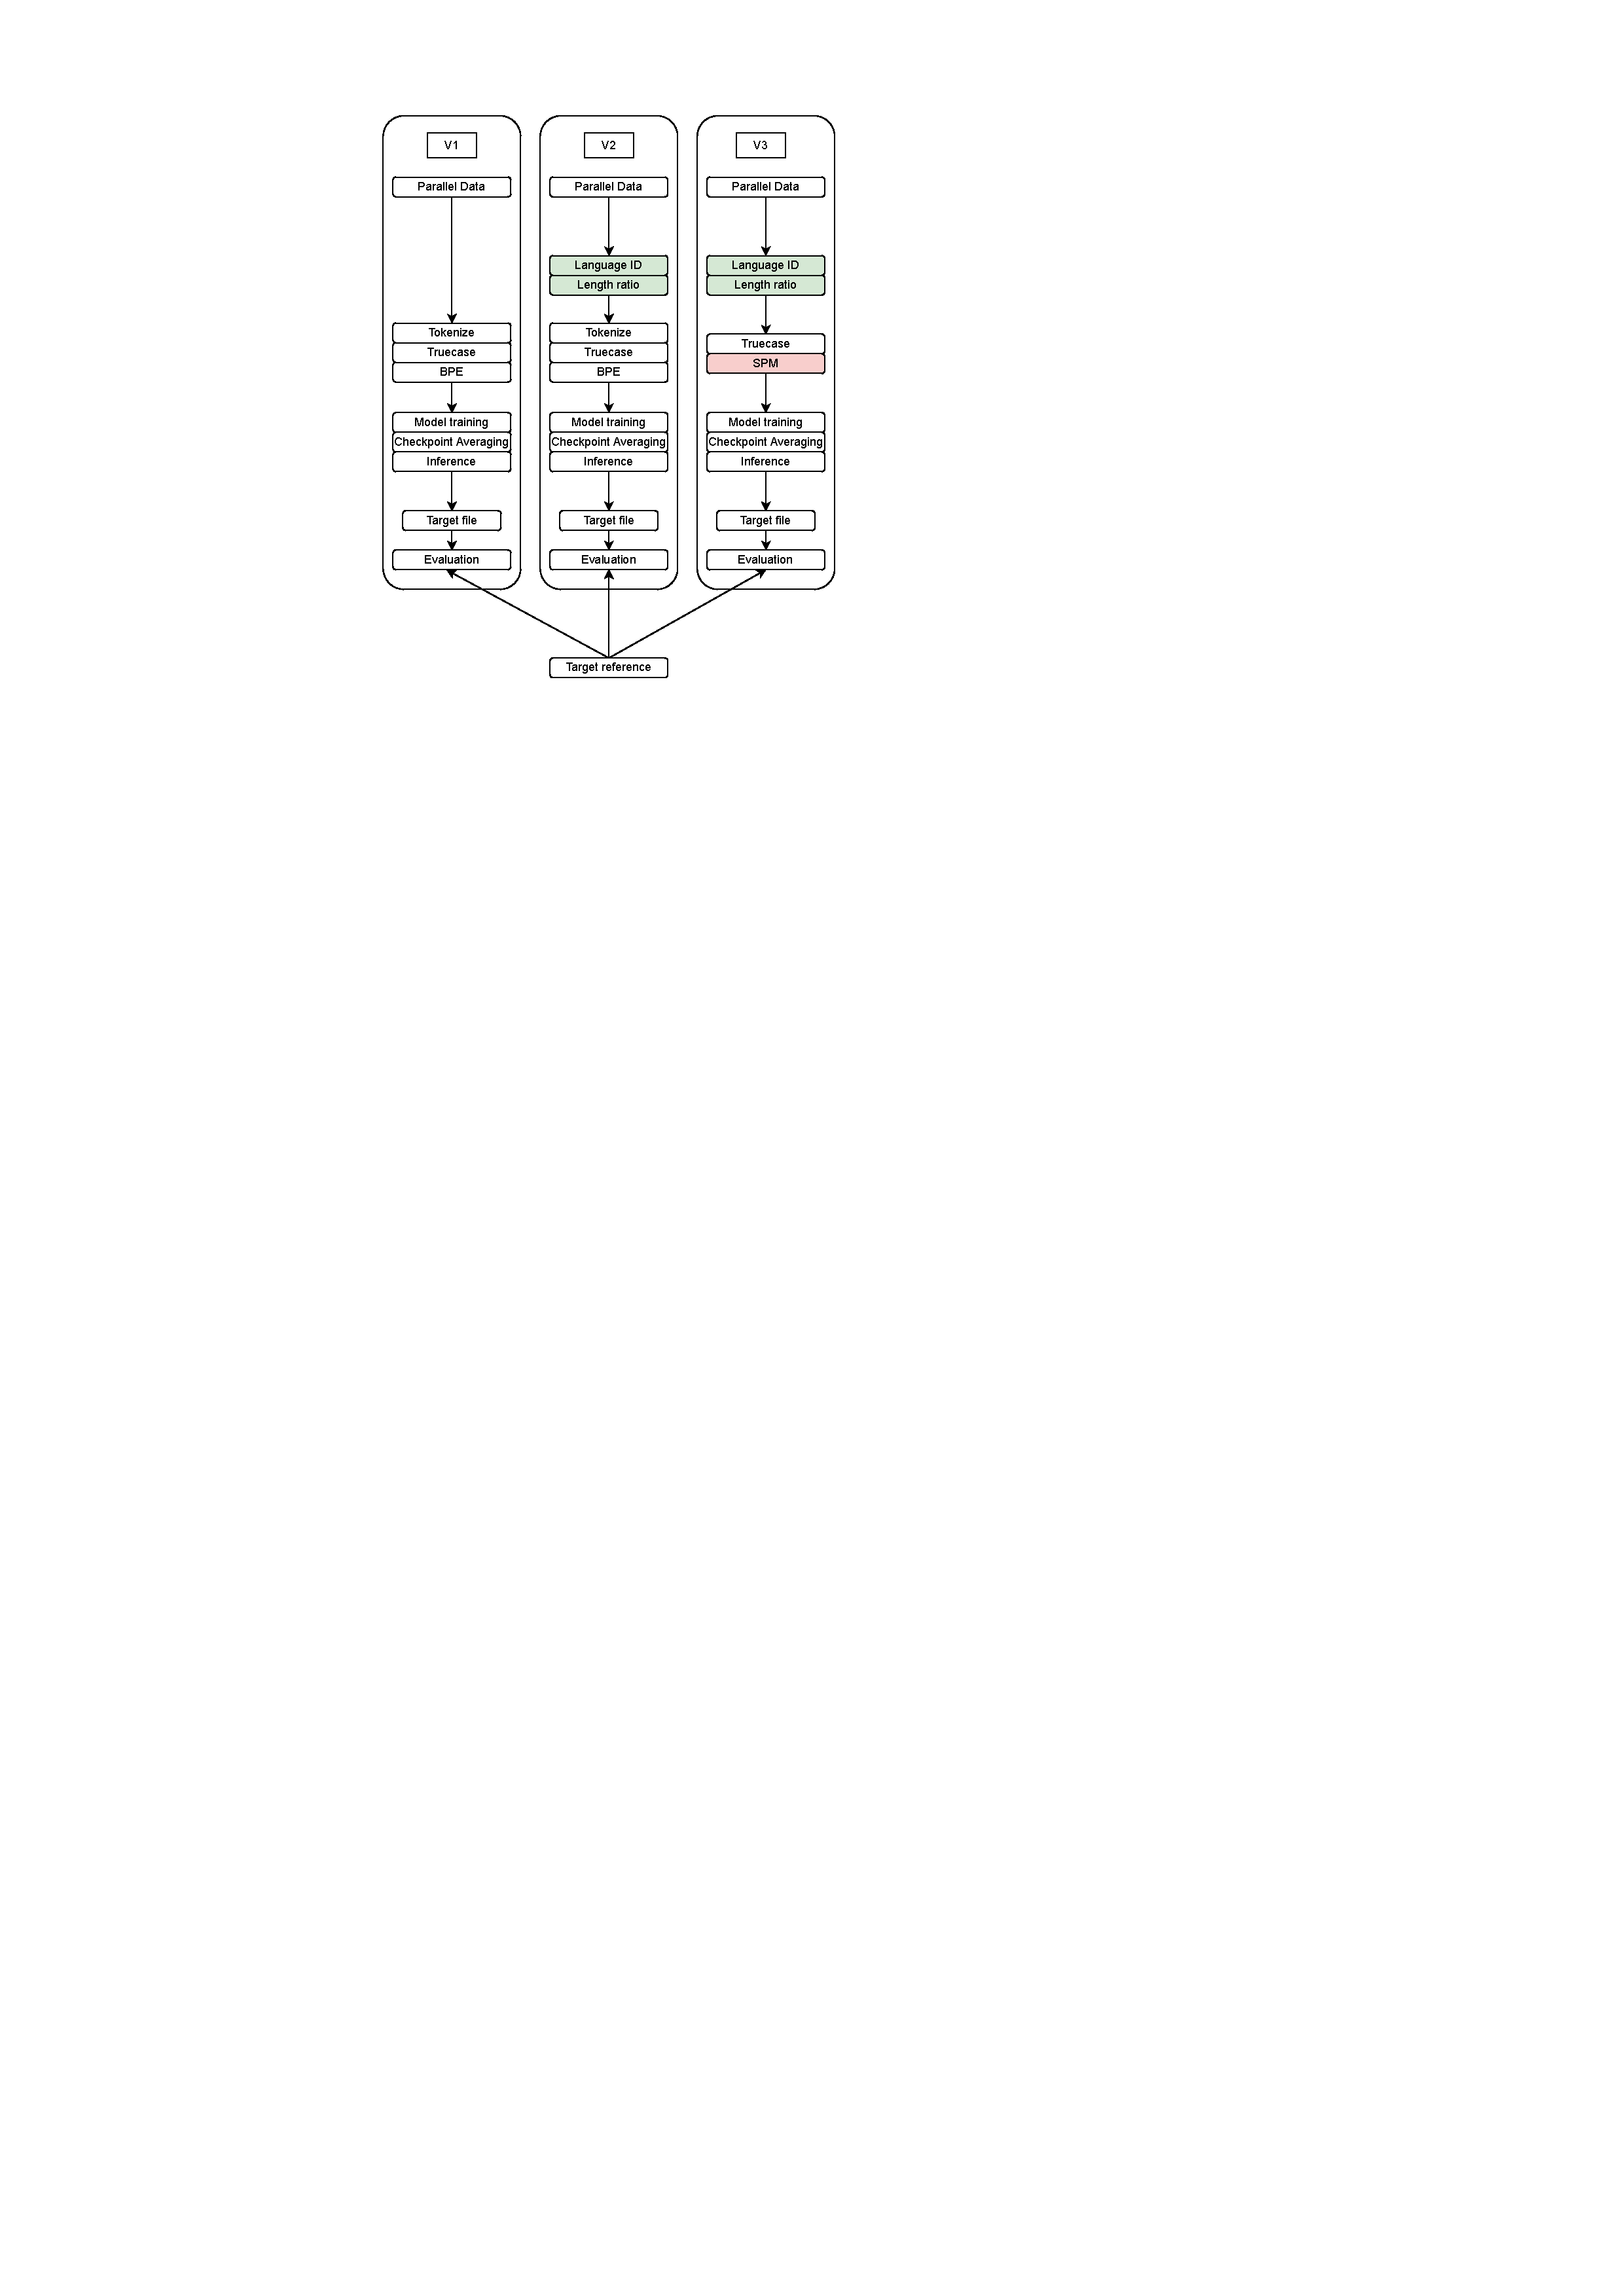
\includegraphics[scale=0.75]{../memoria/resources/pipelinev3.png}


\cp
\section*{Offline systems}
\vspace*{10mm}
\subsection*{General Domain Results}
\vspace*{5mm}
\setlength{\tabcolsep}{12pt}
\begin{table}[H]
\centering
\scalebox{1}{
\begin{tabular}{l|cc}
	System					&	\multicolumn{2}{|c}{BLEU}	\\
								&	WMT13			&	WMT14			\\	\hline
    V0					&\textbf{34.8}				&40.8				\\
	V1							&32.1	&39.1				\\
	V2							&32.6	&39.4	\\
    V3							&34.0				&\textbf{41.0}				\\
%    V4							&34.0				&40.9				\\
\end{tabular}
}
\end{table}
\subsection*{In-Domain Results}
\vspace*{5mm}
\begin{table}[!ht]
\centering
\scalebox{1}{
\begin{tabular}{l|cc}
	System					&	\multicolumn{2}{|c}{BLEU}	\\
								&	CN21			&	CN22			\\	\hline
	V0 &37.2				&37.7				\\
    V3							&\textbf{38.3}	&\textbf{38.7}	\\
%    V4							&\textbf{38.6}				&\textbf{38.8}				\\
\end{tabular}
}
\end{table}

\cp
\section{Domain Adaptation}
\vspace*{10mm}
\subsection*{Backtranslations}
\vspace*{5mm}
\begin{itemize}\itemsep=5mm
	\item Translate monolingual text in the target language to the source language
		\begin{itemize}
			\item Construct a synthetic parallel corpus
		\end{itemize}
	\item Leverage monolingual data in the target language and domain of interest
    \item CERN Document Server monolingual resource $\to$ 1.4M French sentences  
    \item Add syntethic parallel data to training corpus
\end{itemize}

\subsection*{General and In-Domain Results}
\begin{table}[ht]
\centering
\begin{tabular}{l|c|c|c|c}\label{transformer:wmt:r}
System & WMT13 & WMT14 & CN21 & CN22 \\
\hline
V0 & \textbf{34.8} & 40.8 & 37.2 & 37.7\\
V3 & 34.0 & \textbf{41.0} & 38.3 & 38.7\\
V4 & 34.0 & 40.9 & \textbf{38.6} & \textbf{38.8}\\
%v3FTk100 & - & - & 42.0 & \textbf{43.1}\\
%v4FTk100 & - & - & \textbf{42.3} & 42.9\\
\end{tabular}
\label{table:bleuoffv4}
\end{table}


\cp
\section*{Domain Adaptation}
\vspace*{10mm}
\subsection*{Fine-Tuning}
\vspace*{5mm}
\begin{itemize}\itemsep=7mm
	\item A model trained for a general task is used in a specific task or domain
	\item We modify the model parameters to \textit{adapt} it to the domain using in-domain data
    \item Two different fine-tunings of our models
        \begin{itemize}
            \item CERN News training data 
            \item CDS Backtranslations
        \end{itemize}
\end{itemize}

\cp
\section*{Domain Adaptation}
\subsection*{Finetuning Results}
\centering
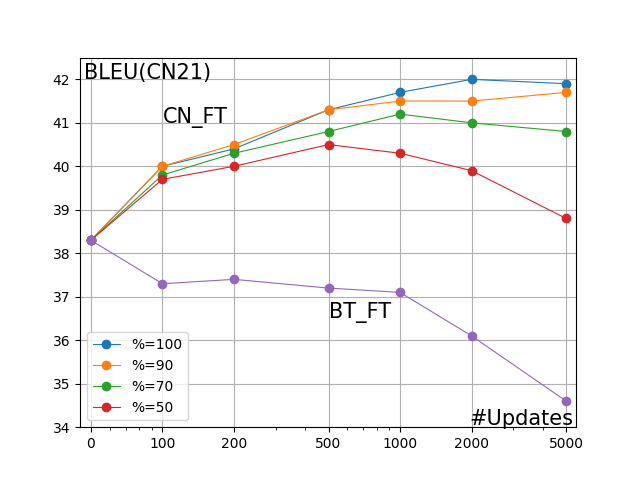
\includegraphics[scale=0.85]{../memoria/resources/CN21_bleu.png}

\begin{itemize}
    \item Best in-domain results at 2000 finetuning updates achieved with CERN News training set 
\end{itemize}
\begin{table}[ht]
\centering
\begin{tabular}{l|c|c}
System & CN21 & CN22 \\
\hline
V0 & 37.2 & 37.7\\
V3FTk100 & 42.0 & \textbf{43.1}\\
V4FTk100 & \textbf{42.3} & 42.9\\
\end{tabular}
\label{table:bleuft}
\end{table}


%%%%%%%%%%%%%%%%%%%%%%%%%%%%%%%%%
% STREAMING MT: FORMALIZATION AND CONTEXT
%%%%%%%%%%%%%%%%%%%%%%%%%%%%%%%%%

\cp
\section{Streaming MT}
\vspace*{10mm}
\begin{itemize}
	\item To simultaneously translate $\mathbf{x}$ into the target $\mathbf{\hat{y}}$, we find the best translation by
\end{itemize}
\vspace*{5mm}
\begin{equation}\nonumber
	\mathbf{\hat{y}} = \argmax_{\mathbf{y} \in \mathcal{Y^*}} p_g(\mathbf{y} \mid \mathbf{x}) = \argmax_{\mathbf{y} \in \mathcal{Y^*}} \prod_t p(y_t \mid \mathbf{x}_{\leq g(t)}, \mathbf{y}_{<t}).
\end{equation}
\vspace*{5mm}
\begin{itemize}\itemsep=5mm
	\item The model only has access to a prefix of the full source to translate
	\item It needs a \textit{policy} $g$ to decide when to perform a reading or writing action
\end{itemize}
\renewcommand{\arraystretch}{1.6}
\vspace*{5mm}
\begin{table}[H]
\centering
\scalebox{0.7}{
\begin{tabular}{r||l}
%	Source 					& Hay libros que valen la pena volver a leer. \\
%	Reference				& Some books are worth reading again. \\ \hline
	Offline					& Hay libros que valen la pena volver a leer. \\
			 					& \textcolor{red}{\textit{\small wait whole sentence}}\hspace*{8cm} There are books that are worth reading again. \\ \hline
	Simultaneous 		& Hay libros \hspace*{2cm} que \hspace*{1cm} valen \hspace*{2cm} la  \hspace*{1.2cm} pena \hspace*{0.9cm} volver \hspace*{1.6cm} a  \hspace*{2.5cm} leer. \\
								& \textcolor{red}{\textit{\small wait 2 words}} There \hspace*{1cm} are \hspace*{1.8cm}  books \hspace*{0.6cm}  that \hspace*{1.5cm} are \hspace*{1.7cm} worth \hspace*{0.6cm} reading \hspace*{1cm} again. \\ 
\end{tabular}
}
\end{table}
\renewcommand{\arraystretch}{1}

%%%%%%%%%%%%%%%%%%%%%%%%%%%%%%%%%
% STREAMING MT: WAIT-K AND LATENCY EVALUATION
%%%%%%%%%%%%%%%%%%%%%%%%%%%%%%%%%
\cp
\section*{Streaming MT}
\vspace*{10mm}

\subsection*{Wait-$k$ Policy}
\vspace*{5mm}
\begin{itemize}\itemsep=5mm
	\item The model reads $k$ tokens before emitting translations
	\begin{itemize}
		\item Afterwards, it alternates between writing and reading operations
	\end{itemize}
\end{itemize}
\begin{figure}[!htp]
\centering
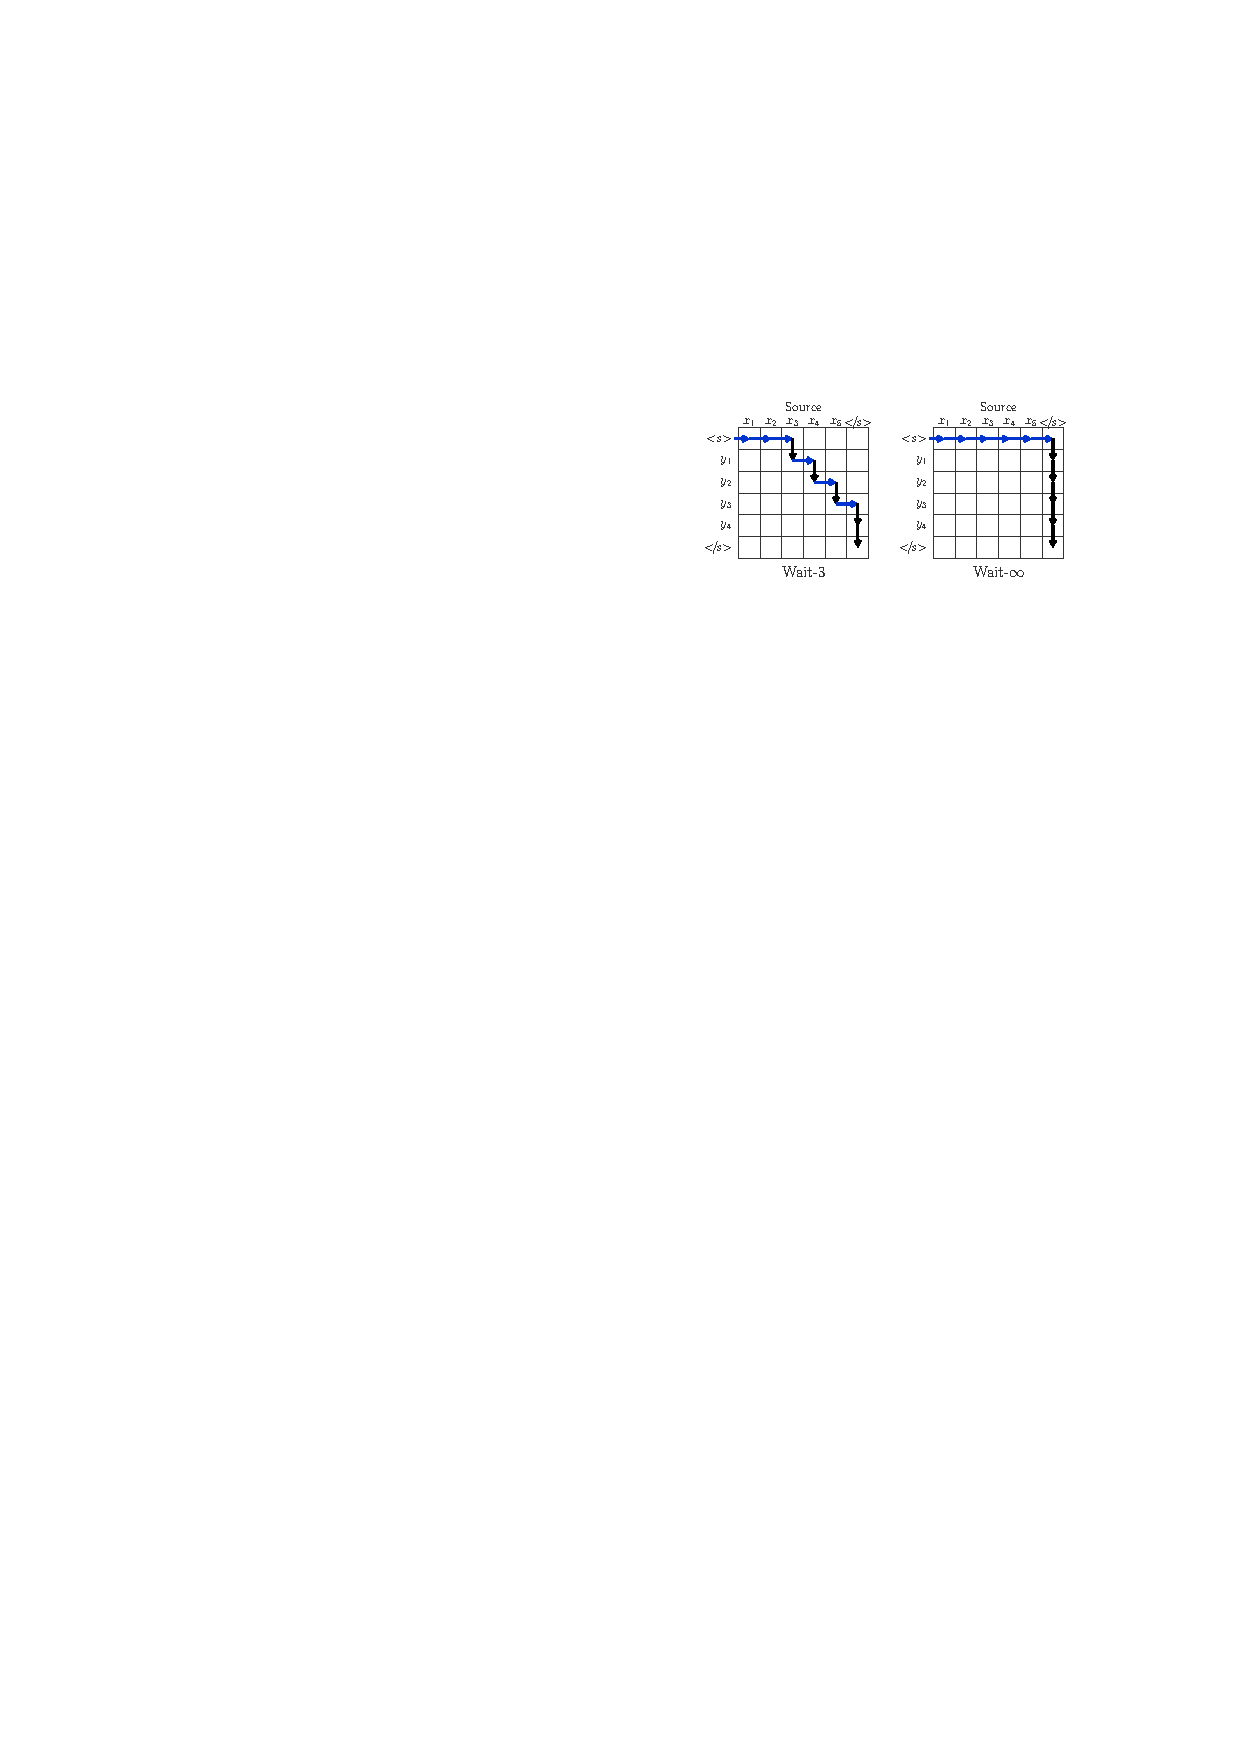
\includegraphics[trim=0.1cm 0.1cm 0.1cm 0.4cm, scale=2.5, clip]{figures/elbayad2020-waitk}
\end{figure}
\begin{itemize}
	\item \empha{Multi-Path Wait-$k$}: simultaneous MT training scheme that considers different values for $k$
\end{itemize}

%%%%%%%%%%%%%%%%%%%%%%%%%%%%%%%%%
% STREAMING MT: WAIT-K FIGURES AND LATENCY EVAL
%%%%%%%%%%%%%%%%%%%%%%%%%%%%%%%%%
\cp
\section*{Streaming MT}
\vspace*{10mm}
\subsection*{Latency Evaluation}
\vspace*{5mm}
\begin{itemize}\itemsep=5mm
	\item Automatic evaluation of latency, independent from hardware and environment 
\vspace*{5mm}
    \item Based on the number of source words available when producing the $t$'th target word 
\vspace*{5mm}
	\begin{itemize}\itemsep=5mm
        \item \empha{AP: Average Proportion} $\to$ Average policy value among all writing times 
        \item \empha{AL: Average Lagging} $\to$ Does not account for the cost of writing operations     
        \item \empha{DAL: Differentiable Average Lagging} $\to$ Accounts for the cost of writing operations
	\end{itemize}
\vspace*{5mm}
    \item \empha{AL} and \empha{DAL} are grounded on the idea of counting how many words the system falls behind a speaker being live translated
\end{itemize}
\vspace*{2cm}

%%%%%%%%%%%%%%%%%%%%%%%%%%%%%%%%%
% RESULTS: SIMULTANEOUS TRANSLATION
%%%%%%%%%%%%%%%%%%%%%%%%%%%%%%%%%

\cp
\section*{Streaming MT}
\vspace*{5mm}
\subsection*{Latency Results}
\vspace{-7.5mm}
\begin{figure}[htp]
\begin{subfigure}{.5\textwidth}
\centering
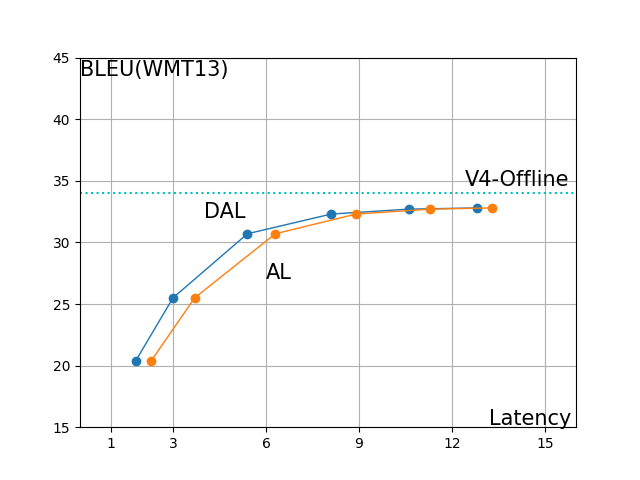
\includegraphics[scale=0.8]{../memoria/resources/onlineres.png}
\end{subfigure}
\begin{subfigure}{.5\textwidth}
\centering
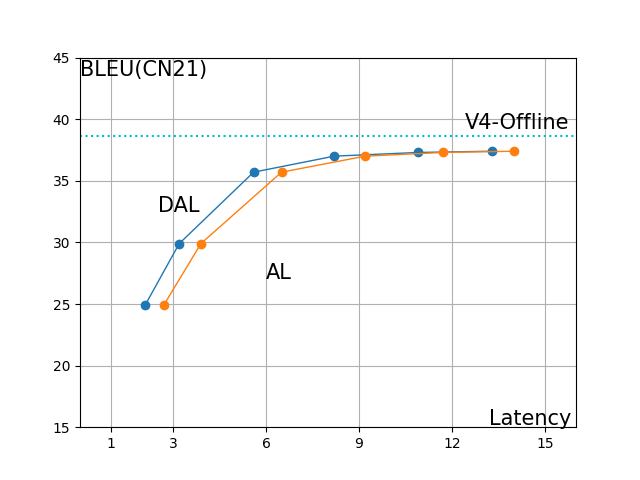
\includegraphics[scale=0.8]{../memoria/resources/onlineresCN.png}
\end{subfigure}
\end{figure}
\begin{itemize}
	\item V4 Multi-Path Wait-$k$ with $k = 6$ at inference time
\end{itemize}
\begin{table}[ht]
\centering
\begin{tabular}{l|c|c|c|c}
    Multi-k & WMT13 & WMT14 & CN21 & CN22 \\
\hline
    BLEU & 30.7 & 36.2 & 35.7 & 35.9 \\
    \hline
    AP & 0.8 & 0.7 & 0.7 & 0.7 \\
    AL & 5.4 & 5.5 & 5.6 & 5.5 \\
    DAL & 6.3 & 6.4 & 6.5 & 6.5 \\
\end{tabular}
\label{table:testres}
\end{table}

%%%%%%%%%%%%%%%%%%%%%%%%%%%%%%%%%
% CONCLUSION & FUTURE WORK
%%%%%%%%%%%%%%%%%%%%%%%%%%%%%%%%%

\cp
\section{Conclusions}
\vspace*{5mm}
\subsection*{Achieved Goals}
\begin{itemize}\itemsep=5mm
	\item State of the art offline and simultaneous NMT were studied
    \item Different data processing techniques were assessed 
    \item A parallel dataset to train and evaluate NMT systems was compiled from CERN News 
	\item In-domain MT systems improved general-domain systems by a relative 12.9\%
    \item Streaming MT systems were developed and evaluated in terms of the trade-off between accuracy and latency
    \item Offline and online MT were built systems to be integrated on CERN premises
\end{itemize}

\subsection*{Future work}
\begin{itemize}\itemsep=5mm
	\item Deployment of MT systems on CERN premises
	\item Domain adaptation for simultaneous MT systems
	\item Study of alternative fine-tuning techniques to perfor domain-adaptaion 
    \item Compilation of new in-domain datasets 
\end{itemize}

%%%%%%%%%%%%%%%%%%%%%%%%%%%%%%%%%
% SAME AS START
%%%%%%%%%%%%%%%%%%%%%%%%%%%%%%%%%
\cp
\thispagestyle{empty}

\begin{center}

\centerline{
\includegraphics[height=0.15\textheight]{figures/UPV-logo}}

\rule{0mm}{20mm}
\Large{\setstretch{1.5}\Large\textbf{\color{darkred}\title}}

\rule{0mm}{30mm}
{\normalsize \color{greyblue}\author}

\newcolumntype{Y}{>{\centering\arraybackslash}X}
\rule{0mm}{0mm}
\begin{table}[ht!]
    \begin{tabularx}{\textwidth}{YY}
        \small \color{greyblue} Jorge Civera Saiz & \small \color{greyblue} Javier Iranzo Sánchez\\
    \end{tabularx}
\end{table}

\end{center}

\centerline{
\includegraphics[height=0.12\textheight]{figures/MLLP_Brand} \qquad \qquad 
\includegraphics[height=0.15\textheight]{figures/vrain.png}}

\normalsize\small
\vspace{10mm}

\centerline{\today}
\vfill

%%%%%%%%%%%%%%%%%%%%%%%%%%%%%%%%%%%%%%%%%%%%%%%%%%%%%%%%%%%%%%%%%%%%%%%%%%%%%%%%%%%%%%%%%%%%%%%%%%
%%%%%%%%%%%%%%%%%%%%%%%%%%%%%%%%%%%%%%%%%%%%%%%%%%%%%%%%%%%%%%%%%%%%%%%%%%%%%%%%%%%%%%%%%%%%%%%%%%
%%%%%%%%%%%%%%%%%%%%%%%%%%%%%%%%%%%%%%%%%%%%%%%%%%%%%%%%%%%%%%%%%%%%%%%%%%%%%%%%%%%%%%%%%%%%%%%%%%

%%%%%%%%%%%%%%%%%%%%%%%%%%%%%%%%%
% ADDITIONAL MATERIAL: TRANSFORMER ENCODER-DECODER
%%%%%%%%%%%%%%%%%%%%%%%%%%%%%%%%%
\cp
\thispagestyle{empty}
\section*{Appendix}
\vspace*{10mm}
\subsection*{Transformer Encoder-Decoder Units}
\begin{figure}[ht]
    \centering
    \subfloat[\centering]{{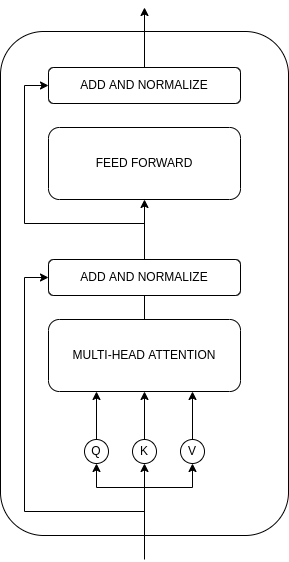
\includegraphics[width=6cm,height=12cm]{../memoria/resources/encode.png} }}%
    \qquad
    \subfloat[\centering]{{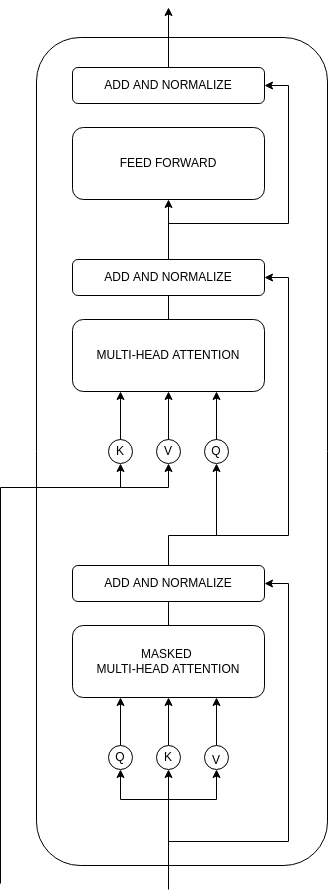
\includegraphics[width=7cm,height=14cm]{../memoria/resources/decode.png} }}%
\end{figure}

%%%%%%%%%%%%%%%%%%%%%%%%%%%%%%%%%
% ADDITIONAL MATERIAL: BLEU TER CHRF
%%%%%%%%%%%%%%%%%%%%%%%%%%%%%%%%%
\cp
\thispagestyle{empty}
\section*{Appendix}
\vspace*{10mm}
\subsection*{Quality Evaluation}
\vspace*{5mm}
\subsubsection*{BLEU}
\begin{equation}\nonumber
	BLEU(4) = BrevityPenalty \times AveragePrecision(4) 
\end{equation}

\begin{equation}\nonumber
	BrevityPenalty = \left\{
		 \begin{array}{ll}
		 	1 & \quad |output| > |reference|	\\
		 	\exp\bigg (1 - \frac{|output|}{|reference|}\bigg) & \quad |output| \leq |reference|
   		 \end{array}
    \right.	
\end{equation}

\begin{equation}\nonumber
	AveragePrecision(N) = \frac{1}{N} \sum_{n=1}^N log p_n, \qquad 	p_n = \frac{\mbox{matching n-grams}}{\mbox{total n-grams in output}}
\end{equation}

%%%%%%%%%%%%%%%%%%%%%%%%%%%%%%%%%
% ADDITIONAL MATERIAL: WAIT-K
%%%%%%%%%%%%%%%%%%%%%%%%%%%%%%%%%
\cp
\thispagestyle{empty}
\section*{Appendix}
\vspace*{10mm}
\subsection*{Simultaneous Translation}
\vspace*{5mm}
\begin{itemize}
	\item $g(i)$ is the number of source tokens read when writing a translation at position $i$.
\end{itemize}
\subsubsection*{Wait-$k$}
\begin{equation}\nonumber
	g_{\text{wait}-k}(i) = \floor*{k+\frac{i-1}{\gamma}}, \qquad	\gamma=\mathbb{E}\big[\gamma_n\big], 	\qquad \gamma_n = \frac{|\mathbf{y}_n|}{| \mathbf{x}_n|}.
\end{equation}

\subsubsection*{Multi-Path Wait-$k$}
For one  wait-$k$ path $\mathbf{z}_{<i}^k$:
\begin{equation}\nonumber
p(\mathbf{y} \mid \mathbf{x}, \mathbf{z}^k) = \prod_i p(y_i \mid \mathbf{x}_{\leq \mathbf{z}_i^k}, \mathbf{y}_{<i}, \mathbf{z}_{<i}^k).
\end{equation}\nonumber
We optimize over multiple wait-$k$ paths:
\begin{equation}\nonumber
\mathbb{E}_K[p(\mathbf{y} \mid \mathbf{x}, \mathbf{z}^k)] \approx \prod_{k \sim \mathcal{U}(K)} p(\mathbf{y} \mid \mathbf{x}, \mathbf{z}^k).
\end{equation}

%%%%%%%%%%%%%%%%%%%%%%%%%%%%%%%%%
% ADDITIONAL MATERIAL: AP, AL, DAL
%%%%%%%%%%%%%%%%%%%%%%%%%%%%%%%%%

\cp
\thispagestyle{empty}
\section*{Appendix}
\vspace*{10mm}
\subsection*{}
\vspace*{5mm}
\subsubsection*{Average Proportion}
\begin{equation}\nonumber
	AP = \frac{1}{|\mathbf{x}| |\mathbf{y}|} \sum_{i=1}^{\mathbf{y}} g(i)
\end{equation}

\subsubsection*{Average Lagging}
\begin{equation}\nonumber
	AL_g = \frac{1}{\tau} \sum_{i=1}^{\tau} \bigg(g(i) - \frac{i - 1}{\gamma}\bigg), \qquad \tau = \tau_g(| \mathbf{x} |) = \min_{i : g(i) = |\mathbf{x}|} i
\end{equation}

\subsubsection*{Differentiable Average Lagging}
\begin{equation}\nonumber
	DAL_d = \frac{1}{| \mathbf{y} |} \sum_{i=1}^{| \mathbf{y} |} \bigg(g_d\prime(i) - (i-1)d \bigg), \qquad d = \frac{1}{\gamma} = \frac{| \mathbf{x} |}{| \mathbf{y} |}
\end{equation}
\begin{equation}\nonumber
g_d\prime(i) = \left\{
		\begin{array}{ll}
			g(i) & \quad i = 1\\
			\max \bigg( g(i), g_d\prime(i-1)+d\bigg) & \quad i > 1\\
		\end{array}
	\right.
\end{equation}

\end{document}
